\documentclass{standalone}
\usepackage{tikz}
\usepackage{ctex,siunitx}
\setCJKmainfont{Noto Serif CJK SC}
\usepackage{tkz-euclide}
\usepackage{amsmath}
\usetikzlibrary{patterns, calc,3d}
\usetikzlibrary {decorations.pathmorphing,decorations.pathreplacing,decorations.shapes}
\begin{document}
\small
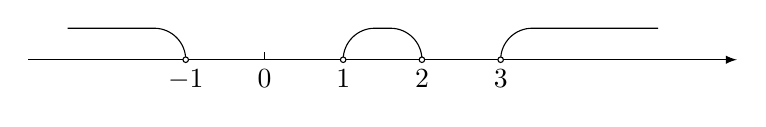
\begin{tikzpicture}[>=latex,scale=1.0]
  \draw[->](-3,0)--(6,0);
  \draw(1,0)arc(180:90:0.4)--(1.6,0.4)arc(90:0:0.4);
  \draw(-1,0)arc(0:90:0.4)--(-2.5,0.4);
  \draw(3,0)arc(180:90:0.4)--(5,0.4);
  \foreach \x in {-1,1,2,3}
    {\draw[fill=white](\x,0)node[below]{$\x$}circle(1pt); }
  \draw[very thin](0,0)node[below]{$0$}--(0,0.1);
\end{tikzpicture}
\end{document}